\documentclass[11pt, oneside]{article}  
% \documentclass[fleqn,10pt]{wlpeerj}


\usepackage{geometry}  
%\usepackage{nunito}
\usepackage{cmbright}
\geometry{letterpaper}   
\usepackage{cite}
\usepackage{graphicx}				% Use pdf, png, jpg, or eps§ with pdflatex; use eps in DVI mode
								% TeX will automatically convert eps --> pdf in pdflatex	
\usepackage{tcolorbox}
\usepackage{amssymb}
\usepackage{longtable}
\usepackage{amsmath}
\usepackage{booktabs}
% \usepackage{emoji}
\usepackage{url}
\usepackage{color}
\definecolor{c1}{rgb}{0.12, 0.56, 1.0}
%SetFonts
\usepackage{xspace}
\usepackage{xcolor}
\usepackage{caption}
\usepackage{subcaption}
\usepackage{authblk} 

\usepackage{sectsty} 
\definecolor{cool_blue}{RGB}{24, 132, 193}
\sectionfont{\color{c1}\selectfont}
\subsectionfont{\color{c1}\selectfont}
\subsubsectionfont{\color{c1}\selectfont}
% \paragraphfont{\color{gray}\selectfont}
\subparagraphfont{\color{gray}\selectfont}

\definecolor{fruitpushorange}{RGB}{255, 127, 0}
\newcommand{\data}{$(s_1, ..., s_k)$\xspace}

\usepackage{soul}
\DeclareRobustCommand{\cms}[1]{ {\begingroup\sethlcolor{fruitpushorange}\hl{(cms:) #1}\endgroup} }
%SetFonts

\sloppy 

\title{
Bi-objective trail-planning for a robot-team orienteering in a hazardous environment
}
\author[1]{Cory M. Simon}
\author[2]{Jeffrey Richley}
\author[2]{Lucas Overbey}
\author[2]{Darleen Perez-Lavin}
\affil[1]{School of Chemical, Biological, and Environmental Engineering. Oregon State University. Corvallis, OR. USA.}
% \affil[]{\texttt{cory.simon@oregonstate.edu}}
\affil[2]{Naval Information Warfare Center Atlantic. Charleston, SC. USA.}
% \corrauthor[1]{Cory M. Simon}{cory.simon@oregonstate.edu}

% \keywords{Keyword1, Keyword2, Keyword3}



%\flushbottom
% \maketitle
%\thispagestyle{empty}


%\affil[*]{}
% \date{}							% Activate to display a given date or no date

\begin{document}
\maketitle

\begin{abstract}
Teams of mobile [aerial, ground, or aquatic] robots have applications in resource delivery, patrolling, information-gathering, pesticide application to crops, forest fire fighting, chemical plume source localization and mapping, and search-and-rescue.
Robot teams traversing hazardous environments---with e.g.,\ rough terrain or seas, strong winds, or adversaries capable of attacking robots---should plan and coordinate their trails in consideration of risks of failure, disablement, or destruction.
Specifically, the robots should take the safest trails, coordinate their trails to cooperatively achieve the team-level objective with robustness to robot failures, and balance the utility from visiting locations against risks of robot losses.

Herein, we consider bi-objective trail-planning for a robot team orienteering in a hazardous environment.
A team of robots are mobile within a hazardous environment, abstracted as a graph whose (i) nodes offer rewards to the team depending on the number of robot visitations and (ii) edges present known probabilities of robot destruction when traversed.
We wish to search for the Pareto-optimal robot-team trail plans that maximize two [conflicting] team objectives: the expected (i) reward and (ii) number of robots that survive the mission. 
A human decision-maker can then select the trail plans that balance, according to their values, reward and robot survival.
We implement ant colony optimization, guided by heuristics, to search for the Pareto-optimal set of robot team trail plans. 
As a case study, we illustrate with an information-gathering mission in a nuclear power plant from a Defense Advanced Research Projects Agency (DARPA) robots challenge.

\end{abstract}

\clearpage


\section{Introduction}
\subsection{Applications of a team of mobile robots}
Mobile [aerial, ground, or aquatic] robots equipped with sensors, actuators, and/or cargo have applications in agriculture (eg. planting and harvesting crops, spraying pesticide, monitoring crop health, destroying weeds) \cite{santos2020path,bawden2017robot}, commerce (eg.\ order fulfillment in warehouses) \cite{wurman2008coordinating}, the delivery of goods \cite{coelho2014thirty}, search-and-rescue \cite{queralta2020collaborative}, chemical, biological, radiological, or nuclear incident response (eg.\ safely localizing the source(s) and mapping the distribution of the hazard) \cite{murphy2012projected,hutchinson2019unmanned}, environmental monitoring \cite{dunbabin2012robots,hernandez2012mobile,yuan2020maritime}, safety monitoring and leak detection in industrial chemical plants \cite{soldan2014towards,francis2022gas}, forest fire monitoring and fighting \cite{merino2012unmanned}, target tracking \cite{robin2016multi}, and military surveillance and reconnaissance. 

Deploying a \emph{team} of robots for a mission, as opposed to a single robot, can increase spatial coverage, decrease the time to achieve the objectives, and make achievement of the objectives robust to the failure of robots \cite{schranz2020swarm,brambilla2013swarm}.

We often wish for the team of mobile robots to coordinate their paths in the environment to cooperatively achieve a shared, team-level objective \cite{parker1995design,parker2007distributed}.
For example, consider the team orienteering problem (TOP) \cite{gunawan2016orienteering,vansteenwegen2011orienteering}. 
The environment, in which a team of robots are mobile, is modeled as a graph (nodes: locations; edges: spatial connections between locations). Each node offers a reward to the team if visited by a robot.
The TOP is to plan the paths of the robots between a source and destination node, subject to a per-robot travel budget, to accumulate the most rewards from the graph as a team. The TOP can be formulated as an integer program. Loosely, the OP combines the classic knapsack problem (selecting the nodes from which to collect rewards, under the travel budget) and traveling salesman problem (finding the shortest path that visits these nodes) \cite{vansteenwegen2011orienteering}.

\subsection{Teams of mobile robots orienteering in risky environments} 
In some applications, the team of robots move in a hazardous environment and incur risks of failure, destruction, and/or disablement. 
The risks could originate from dangerous terrain, rough seas, strong winds, lightening, the presence of heat, radiation, or corrosive chemicals, mines, piracy, or an adversary with the capability to attack/disable/destroy robots \cite{agmon2017robotic}. 

Robots traversing a hazardous environment should plan and coordinate their trails in consideration of their risks of failure.
First, the robots should take the safest trails to reach their assigned locations to visit. 
Second, the robots should coordinate their trails so that achievement of the team objective is resilient to robot failures \cite{zhou2021multi}. 
A \emph{resilient} team of robots \cite{prorok2021beyond}
(i)
adopts risk-aware plans that anticipate failures and endow the team with \emph{robustness}---the ability to withstand failures with minimal concession of the objective,
or
(ii) adapt their trail plans in response to realized failures of robots to recoup the loss in the objective due to the failed robots. 
Third, the trail plans must balance the utility gained from visiting different locations in the environment against the risks incurred by the robots to reach those locations.

Models and algorithms have been developed for coordinated robot team orienteering in risky environments abstracted as graphs \cite{zhou2021multi}. 
In the Team Surviving Orienteers problem (TSOP) \cite{jorgensen2018team,jorgensen2017matroid,jorgensen2024matroid}, each node of the graph offers a reward to the team when visited by a robot, but each edge traversal by a robot incurs an independent probability of destruction. The objective in the [offline] TSOP is to plan the paths of the robots (from a source to destination node) to maximize the expected team reward under the constraint that each robot survives the mission with a probability above a certain threshold. 
%In the extended Matroid TSO problem \cite{jorgensen2017matroid,jorgensen2024matroid}, we seek to maximize the weighted
%expected number of nodes visited by one or more robots.
Relatedly, the Foraging Route with the Maximum Expected Utility problem \cite{di2022foraging} is to plan the foraging route of a robot collecting rewards in a hazardous environment, but the rewards are lost if the robot is destroyed before returning to the source node to deposit the goods it collected.
In the [offline] Robust Multiple-path Orienteering Problem \cite{shi2023robust}, similarly, each node gives a reward to the team only if a robot visits it and survives the mission; the paths of the $K$ robots are planned to maximize the team reward under the worst-case attacks of $\alpha<K$ of the robots by an adversary. 
Viewed as a two-stage, sequential, one-step game with perfect information, the optimal path plans must trade off (i) redundancy in the nodes visited to give robustness against attacks and (ii) coverage of many nodes to collect many rewards.
Other work involving robot path-planning in hazardous environments includes 
(i) maximizing coverage of an area containing threats to robots \cite{korngut2023multi,yehoshua2016robotic}, 
(ii) handling adversarial attacks on the sensors of the robots \cite{liu2021distributed,zhou2022distributed,mayya2022adaptive,zhou2018resilient}, and 
(iii) gathering information in an environment with unknown hazards \cite{schwager2017multi}.

\subsection{Our contribution}
Inspired by the TSOP \cite{jorgensen2018team,jorgensen2017matroid,jorgensen2024matroid}, we pose the bi-objective team orienteering in hazardous environments problem (BOTOHE), then implement a bi-objective ant colony optimization algorithm, guided by heuristics, to search for the Pareto-optimal robot-team trail plans for an example BOTOHE instance for an information-gathering mission in a nuclear power plant from a Defense Advanced Research Projects Agency (DARPA) robots challenge.

\paragraph{The bi-objective team orienteering in hazardous environments problem (BOTOHE).} 
A team of robots are mobile in a hazardous environment, modeled as a directed graph whose edges present known, independent probabilities of destruction to a robot that traverses them.
The nodes of the graph offer rewards to the team depending on the number of robot-visitations over the mission.
The BOTOHE is to plan the closed trails of the robots to maximize two team-level objectives: the expected
(1) rewards to the team given by the nodes and 
(2) number of robots that survive the mission. 
(In this offline setting, the trails are set at the beginning of the mission, then followed by the robots without adaptation.)
See Fig.~\ref{fig:overview}.

\paragraph{Intuition.} Three interesting features of the BOTOHE are: 
(1) for the survival objective, the robots seek the safest closed trails to visit the nodes assigned to them,
(2) for the reward objective, the robot team builds node-visit redundancy into their trail plans to make the team-reward robust to the loss of robots during the mission,
(3) the two objectives are inherently conflicting, as the robots must risk their survival while taking their trails to visit nodes and collect rewards\footnote{Two extremes: (1) to maximize survival, the robots never leave the source node no matter the rewards to be gained and (2) to maximize reward, each robot traverses the entire graph no matter the risks involved.}.

\paragraph{Pareto-optimal trail plans.}
To handle the conflicting objectives, we search for the Pareto-optimal set of robot-team trail plans. By definition, a Pareto-optimal trail plan cannot be altered to give higher expected rewards without lowering the expected number of robots that survive and vice versa. 
Fig.~\ref{fig:pareto_optimal} illustrates.
We then can present the Pareto-optimal set to a human decision-maker who selects the robot-team trail plans that makes some tradeoff between the two objectives, based on his or her value of rewards vs. robot survival. 

\paragraph{Solution approach.} 
We employ a bi-objective ant colony optimization algorithm, guided by a heuristic, to search for the Pareto-optimal set of robot-team trail plans.
{\color{red} say more}
We illustrate by solving a BORTOP instance inspired by information-gathering for illustration.

\begin{figure}[h!]
    \centering
     \begin{subfigure}[b]{0.62\textwidth}
    	\includegraphics[width=\textwidth]{drawings/overview_2.pdf}
	\caption{} \label{fig:overview}
    \end{subfigure}
    \begin{subfigure}[b]{0.66\textwidth}
    	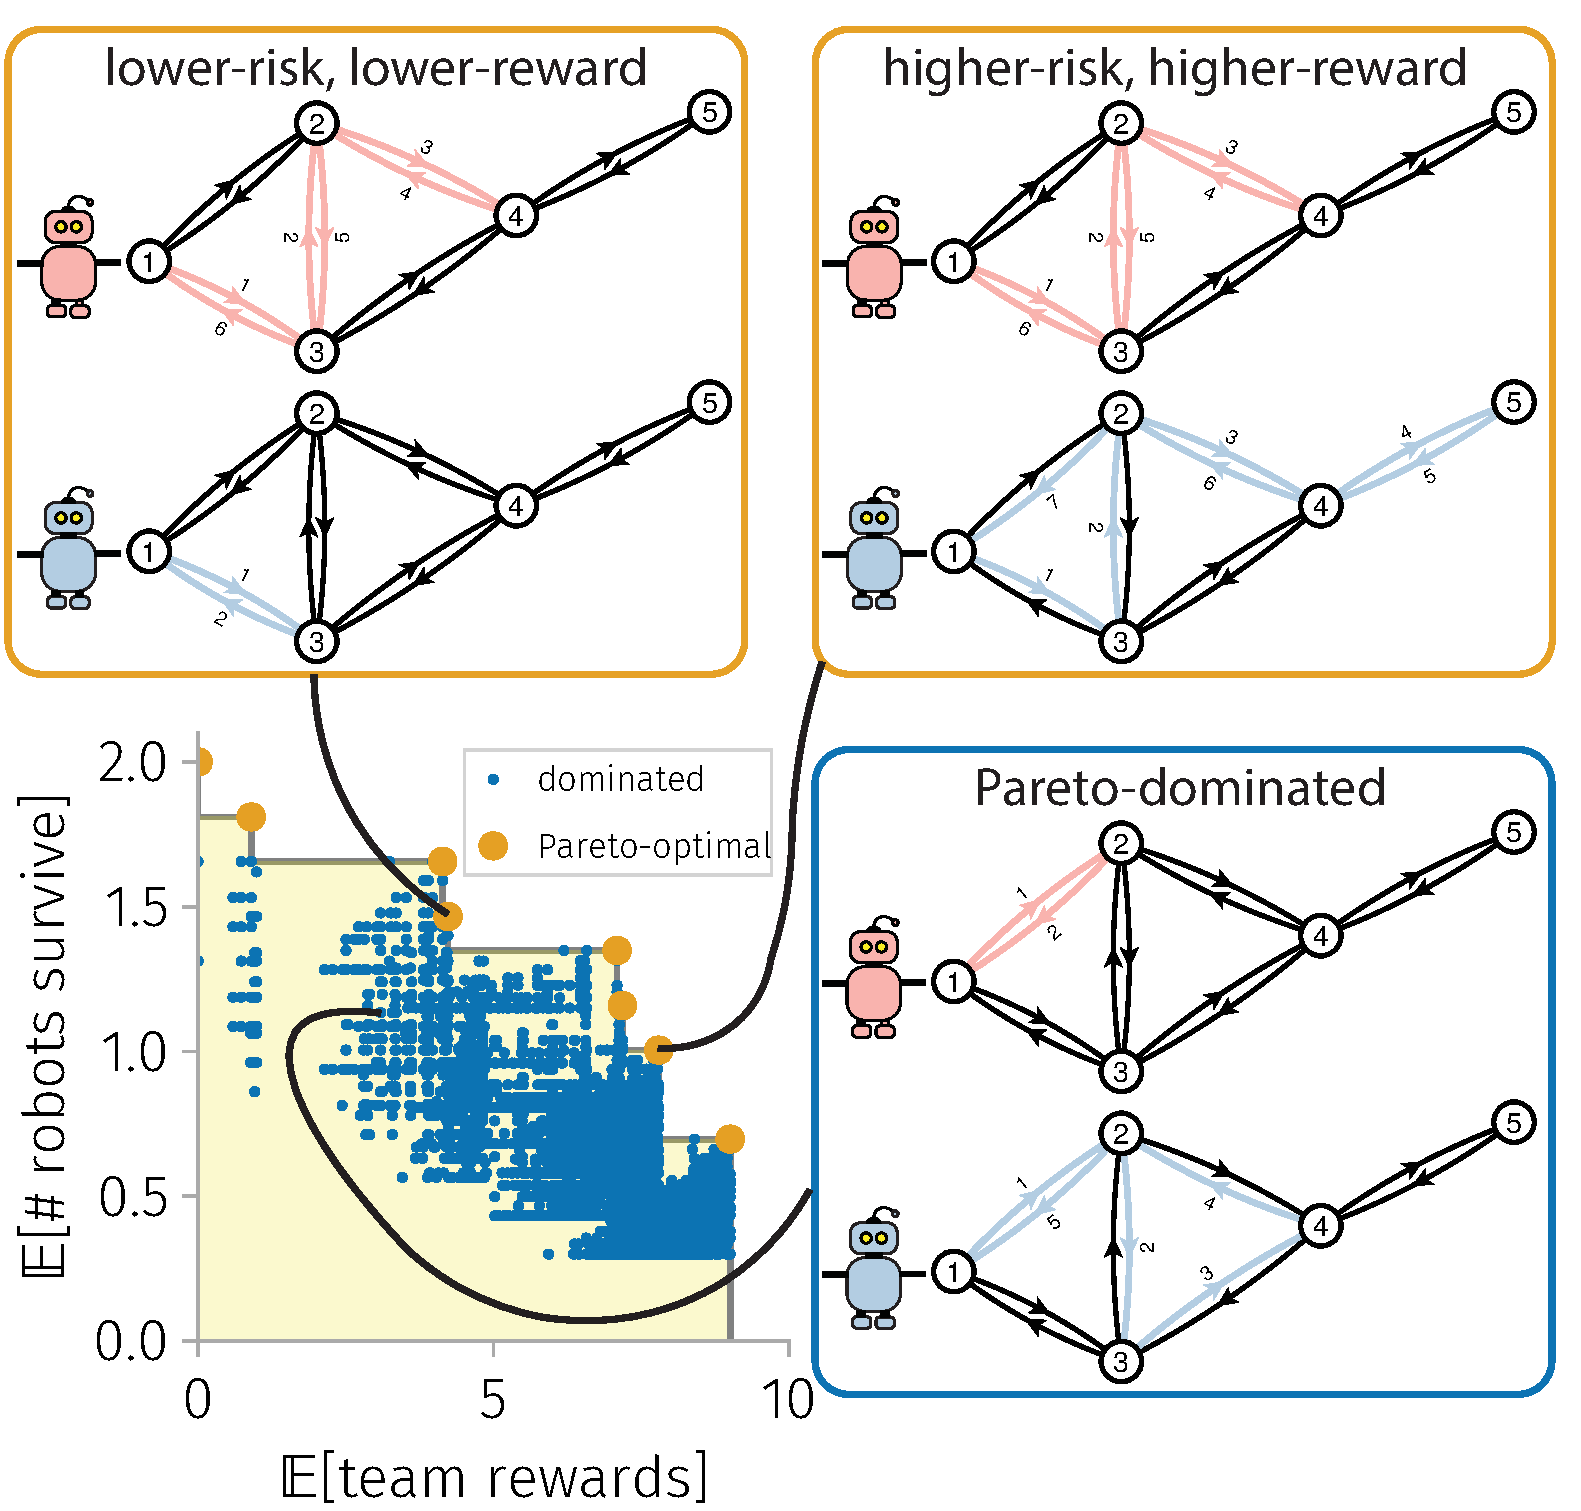
\includegraphics[width=\textwidth]{drawings/toy_pareto_front2.pdf}
	\caption{} \label{fig:pareto_optimal}
    \end{subfigure}
    \caption{
      The bi-objective team orienteering in hazardous environments problem (BOTOHE).
      (a) A team of robots are mobile on a directed graph whose 
      nodes offer a reward to the team e.g.\ if visited by a robot and 
      edges present a probability of destruction to robots that traverse them (tornado = 1/10 probability of destruction). Our task is to plan the trails of the robots to maximize the expected reward collected and the expected number of robots that survive.
      (b) Pareto-optimal and -dominated robot-team trail plans scattered in objective space, with two Pareto-optimal and one Pareto-dominated trail plans shown.}
\end{figure}



\section{The bi-objective team orienteering in hazardous environments problem (BOTOHE)}
%In the risky team orienteering problem (RTOP), our task is to plan the trails of a team of mobile robots on a directed graph whose (i) nodes offer rewards to the team depending on the number of robots that visit them and (ii) edges, when traversed by a robot, impose a risk of robot failure/destruction.
%The trails are set at the beginning of the mission, then followed by the robots without updates during the mission---an offline setting. 
%For the bi-objective RTOP (BO-RTOP), we wish to find the set of Pareto-optimal trail plans for the robot team that maximize the expected (i) rewards collected by the team and (ii) the number of robots that survive the mission.




\subsection{Problem setup}
We pose the bi-objective team orienteering in hazardous environments problem (BOTOHE).

\paragraph{Spatial abstraction of the environment as a directed graph.}
We model the environment as a directed graph $G=(\mathcal{V}, \mathcal{E})$, where $\mathcal{V}$ is its set of vertices and $\mathcal{E}$ is its set of edges (ordered pairs of distinct vertices). We assume $G$ is strongly connected, but not necessarily complete.

\vspace{-\baselineskip}
\subparagraph{Interpretation.} 
Each node $v\in \mathcal{V}$ represents a distinct location in the environment (e.g., a room in a building or a house in a neighborhood).
Each edge $(v, v^\prime) \in \mathcal{E}$ represents a direct spatial connection for traveling from one location $v$ to another $v^\prime$ (e.g., a doorway or a road).


% the best (e.g., shortest or safest) path (in Euclidean space) for a mobile robot to take from the location represented by node $v$ to the location represented by $v^\prime$.
% Note, we do not assume the graph is complete\footnote{Ie., not every pair of distinct nodes $\{v, v^\prime\}$ is joined by two edges $(v, v^\prime)$ and $(v^\prime, v)$. 
% Eg., consider a building with node $v$ representing a room on the first floor, node $v^\prime$ a room on the second floor, and node $u$ as the staircase between the first and second floors. Traveling from node $v$ to node $v^\prime$ necessitates passing through node $u$ first.}.

\paragraph{The team of mobile robots.}
A homogenous team of $K$ robots all begin at a base station represented by node $v_b \in \mathcal{V}$ of the graph $G$. The robots are \emph{mobile} in the environment, meaning they may walk on the graph $G$.
Ie., each robot can sequentially move from one node $v$ to another node $v^\prime$ joined with it via traversing edge $(v, v^\prime)\in\mathcal{E}$.

\paragraph{Team rewards offered by nodes in the graph.}
Each node $v\in \mathcal{V}$ in the graph $G$ offers a reward to the robot team, whose magnitude depends on the number of robots that visit it over the course of the mission. 
The node reward function $r_v: \mathbb{N}_{\geq 0} \rightarrow \mathbb{R}$ maps 
the number of robots that visit node $v$ over the course of the mission
% visits node $v$ receives by a robot over the course of the mission
 to 
 the reward accumulated by the team from node $v$.
 The total reward collected by the team is additive among nodes of the graph.
Note, even if a robot is destroyed after leaving node $v$, it still counts as a successful visit to node $v$.
Ie., the marginal reward offered by a node is immediately and irrevocably accumulated by the team after a robot visit.

\vspace{-\baselineskip}
\subparagraph{Interpretation.} The rewards given by a node represent the utility gained by the team when eg. robots deliver units of a resource to the node, take images of the node and transmit them back to the command center, actuate some process (eg. turn a valve) at the node, etc. 

\vspace{-\baselineskip}
\subparagraph{Remarks.} The reward offered by a node could be negative, ie. there could be a penalty to visit a node instead of an incentive.
Also, unlike in the TSOP, we do not assume the node reward function $r_v$ satisfies a diminishing returns property. E.g., for resource delivery, two deliveries of a resource could be required to construct some useful equipment from which utility is ultimately gained.


\paragraph{The probabilistic model of robot destruction during trail-following.} 
Each robot incurs a risk of destruction when it traverses an edge of the graph $G$.
% following its trail $\rho$. 
Specifically, starting (in a functioning state) at some node $v$, a robot survives with probability $\omega(v, v^\prime)$ the two-step process of (i) traversing edge $(v, v^\prime) \in \mathcal{E}$ then (ii) visiting node $v^\prime$. 
We assume (i) each outcome (survival or destruction) of this two-step process is an independent event and (ii) the survival probabilities are static over the course of the mission. 
Thus, from the function $\omega: \mathcal{E} \rightarrow (0, 1]$ that assigns robot survival probabilities to each edge of the graph $G$, we can compute the survival probabilities of the $K$ robots following any given set of trails.
% plans $\{\rho_1, ..., \rho_K\}$.% and (2) the expected utility of the rewards harvested by the robots along their paths, which we write next. 



\vspace{-\baselineskip}
\subparagraph{Interpretation.} The hazards in the environment could originate from obstacles the robot could crash into, rough terrain or seas, severe weather, mines, or adversaries capable of attacking the robots at the edge and/or sink node.
The stochasticity in the survival/failure of a robot traversing an edge originates from eg. (i) the unpredictability of an aerial robot crashing into an obstacle, a ground robot getting stuck in rocks/mud, or a surface aquatic robot succumbing to ocean waves or (ii) an adversary with an imperfect capability to detect and attack robots.

\vspace{-\baselineskip}
\subparagraph{Possible asymmetry.} We do not assume $\omega$ is symmetric, ie., that $\omega(v, v^\prime) = \omega(v^\prime, v)$. The traversal from node $v$ to $v^\prime$ may be more dangerous than from $v^\prime$ to $v$ owing to eg., (i, asymmetric edge traversal) strong air or water currents in the direction $v^\prime$ to $v$ or (ii, asymmetric dangers at nodes) an adversary with attack capability at node $v^\prime$ but not at $v$. %Even if edge traversal risks are symmetric, the action of visiting a node be risky, and node $v$ may be more or less dangerous than node $v^\prime$, breaking symmetry. 

\paragraph{The robot-team trail plans.}
To collect rewards, each robot on the team will plan to execute/follow a closed, directed trail $\rho$ on the graph $G$.  
The set of closed, directed trails $\mathcal{P}:=\{\rho_1, ..., \rho_K\}$ the robot-team plans to follow constitute the \emph{robot-team trail plans} for the \emph{mission}. These are only ``plans'' because a robot may fail in the process of following its planned trail and thus not actually visit all nodes in its trail plan.

\vspace{-\baselineskip}
\subparagraph{A closed, directed trail.} 
A \emph{directed trail} is an ordered list of nodes $\rho = (\rho[0], \rho[1], ..., \rho[\lvert \rho \rvert])$ where
(i) $\rho[i] \in \mathcal{V}$ is the $i$th node in the trail,  
(ii) an edge exists from each node to the next node, ie., $(\rho[i-1], \rho[i])\in\mathcal{E}$ for $1 \leq i  \leq \lvert \rho \rvert$,
(iii) $\lvert \rho \rvert$ is the number of edges traversed in the trail,
and
(iv) the edges traversed in the trail are unique, ie. each edge in the multiset $\{(\rho[i-1], \rho[i])\}_{i=1}^{\lvert \rho \rvert}$ has a multiplicity of one.
Note, unlike a path, the nodes in a trail are not necessarily distinct \cite{wilson1979introduction}.
A \emph{closed} trail begins and ends at the same node, ie. $\rho [0]=\rho[\lvert \rho \rvert]$, which, here, $=v_b$.

\vspace{-\baselineskip}
\subparagraph{The static/offline setting.} 
The robot-team trail plans $\mathcal{P}$ are set at the beginning of the mission, then followed by the robots without adaptation or updates during the mission (e.g., in reaction to realized robot failures). 
I.e., robots cannot communicate their status to the command center during the mission and/or the command center cannot send updated instructions to the robots after the mission executes.

\paragraph{The bi-objective, risky team orienteering problem.}
Given the graph $G$ as a spatial abstraction of the environment, the node reward functions $\{u_v : v \in\mathcal{V}\}$, the edge survival probability map $\omega$, and a homogenous team of $K$ mobile robots starting at the base node $v_b$, our goal in the \emph{bi-objective, risky team orienteering problem} is to determine the optimal robot-team [closed] trail plans $\mathcal{P}$ that maximize two-objectives, (1) the expected team-reward and (2) the expected number of robots that survive the mission:
\begin{equation}
\max_{\mathcal{P}=\{\rho_1, ..., \rho_K\}} \left( \mathbb{E}[U(\mathcal{P})], \mathbb{E}[R(\mathcal{P})] \right).
\label{eq:the_two_objs}
\end{equation}

\vspace{-\baselineskip}
\subparagraph{Objective \#1: the expected reward collected by the robots.}
Let $T_v(\mathcal{P}) $ be the number of robots on the team with trail plans $\mathcal{P}$ that ultimately visit node $v$.
Because of the stochasticity of robot survival while trail-following, and thus of which nodes in the trail plan each robots ultimately visits, $T_v$ is a random variable.
Then, the total team rewards collected by the robot-team following trail plans $\mathcal{P}$ is also a random variable:
\begin{equation}
U(\mathcal{P}) = \sum_{v\in\mathcal{V}} u_v\left ( T_v(\mathcal{P}) \right).
\end{equation}
We wish to devise robot-team trail plans $\mathcal{P}$ to maximize the expected team reward, $\mathbb{E}[U(\mathcal{P})]]$.

\vspace{-\baselineskip}
\subparagraph{Objective \#2: the expected number of robots that survive the mission.}
Let $R(\mathcal{P})$ be the number of robots, on a robot team with trail plans $\mathcal{P}$, that ultimately survive the mission. Because of the stochasticity of robot survival while trail-following, $R$ is a random variable. We wish to devise robot-team trail plans $\mathcal{P}$ to maximize the expected number of robots that survive the mission, $\mathbb{E}[R(\mathcal{P})] \in (0, K]$.

We derive formulas for the values of the two objectives as a function of the robot-team trail plans later (see eqn.~\ref{eq:formula_obj1} and eqn.~\ref{eq:formula_obj2}). 

\subparagraph{Remarks on lacks of constraints.} 
Unlike in the TSOP formulation, we do not impose constraints on the survival probability of each individual robot. We accept if one [unmanned] robot bears much more risk of destruction than another during the mission. 
Unlike in the TOP formulation, we do not constrain the length of the planned trail of the robots. We assume each robot has sufficient fuel/electrical battery power to traverse the graph.

% TODO merge with above
\subparagraph{Comparison with TSO}
Our BO-RTOP formulation follows the TSOP \cite{jorgensen2018team} with four modifications: we (i) omit the constraints that each robot survives above a threshold probability, (ii) allow robots to follow trails instead of paths and hence allow a robot to visit a given node more than once\footnote{A path prohibits a robot from visiting a node more than once. Unlike trails, restricting to paths prohibits a robot from eg. visiting multiple nodes in a star graph.}, (iii) aim to maximize two objectives instead of one, and (iv) do not assume the reward function is submodular. 




\paragraph{Seeking the Pareto-optimal set of robot-team trail plans.} 
In most problem instances, the bi-objective problem in eqn.~\ref{eq:the_two_objs} presents a conflict between designing the robot-team trail plans that maximize the expected reward vs. the expected number of surviving robots. 
Focusing solely on the second objective, the robots safely stay at the base station and do not attempt to collect any rewards---no matter the [positive] size of the rewards to be gained by leaving the base station. 
Focusing solely on the first objective, each robot plans to traverse the entire graph to attempt to collect each [suppose, positive and single-visit] reward with maximal redundancy for resilience to failures---no matter the risk involved.
In other words, there may not exist a utopian robot-team trail plan that simultaneously maximizes both objectives. 

Given the conflict between the two objectives, the ultimate robot-team trail plans selected for the mission must make a tradeoff between the expected reward and the expected number of robots that survive. 
A human decision-maker must invoke their values to make this tradeoff.
Valuing survival more than rewards will favor trail-plans where robots do not enter dangerous regions of the environment, even if large rewards are offered there. Valuing rewards more than survival will instead send robots into these dangerous regions to attempt collection of those rewards. 

Herein, solving the bi-objective optimization problem in eqn.~\ref{eq:the_two_objs} constitutes finding the Pareto-optimal set of team-robot trail plans. Then, we can present the Pareto set to the decision-maker, who ultimately selects the team-robot trail-plans according to their values placed on team-reward vs. robot survival. 

\paragraph{Pareto-optimal team-robot trail plans.} 
A \emph{Pareto-optimal} \cite{pardalos2017non} robot-team trail plan $\mathcal{P}$ cannot be altered to
(1) increase the survivability objective $\mathbb{E}[R(\mathcal{P})]$ \emph{without} compromising (decreasing) the reward objective $\mathbb{E}[U(\mathcal{P})]$
nor
(2) increase the reward objective $\mathbb{E}[U(\mathcal{P})]$ \emph{without} compromising (decreasing) the survivability objective $\mathbb{E}[R(\mathcal{P})]$.
Formally, team trail plans $\mathcal{P}$ \emph{Pareto-dominate} team trail plans  $\mathcal{P}^\prime$ if both
\begin{align}
	\left (\mathbb{E}[U(\mathcal{P})] \geq \mathbb{E}[U(\mathcal{P}^\prime)]  \right) & \wedge \left( \mathbb{E}[R(\mathcal{P})] \geq \mathbb{E}[R(\mathcal{P}^\prime)] \right) \\
	\left( \mathbb{E}[U(\mathcal{P})] > \mathbb{E}[U(\mathcal{P}^\prime)] \right) & \vee \left( \mathbb{E}[R(\mathcal{P})] > \mathbb{E}[R(\mathcal{P}^\prime)] \right).
\end{align}
Clearly, then, we should never choose Pareto-dominated trail plans $\mathcal{P}^\prime$, regardless of our weight on the two objectives, over the trail plans $\mathcal{P}$. A plan $\mathcal{P}$ belongs to the Pareto-optimal set of plans if no other trail plans Pareto-dominate it. 
See Fig.~\ref{fig:pareto_optimal}.

\subsection{Deriving formulas for the two objectives}
We now derive formulas for the two objectives, the expected team rewards, $\mathbb{E}[U(\mathcal{P})]$ and the expected number of robots that survive the mission $\mathbb{E}[R(\mathcal{P})]$, as a function of the robot-team trail plans $\mathcal{P}$. These formulas follow from the edge survival probability map $\omega$ and node reward functions $\{u_v : v \in \mathcal{V}\}$.

\paragraph{The survival of a single robot along its followed trail.}
Let $S_n(\rho) : \{\text{fail}, \text{survive}\} \rightarrow \{0, 1\} $ be the Bernoulli random variable that is $1$ if a robot following trail $\rho$ survives to visit the $n$th node in this trail, and $0$ if it does not. For the event of survival, the robot must survive its traversal of \emph{all} of the first $n$ edges in its trail. So the probability of survival is:
\begin{equation}
	\pi(S_n(\rho) = 1) = \prod_{i=1}^n \omega(\rho[i-1], \rho[i]) \text{ for } 0 \leq n \leq \lvert \rho \rvert %\in \{1, ..., \lvert \rho \rvert\} 
	\label{eq:pi_S_n}
\end{equation} The factorization owes to the independence of the edge-traversal$+$node-visit survival events.
The complement of the event of survival is failure, so $\pi(S_n(\rho) = 0)=1-\pi(S_n(\rho) = 1)$.

Note, the outcome $S_n(\rho)=0$ implies $S_{n+i}(\rho)=0$ for $1 \leq i \leq \lvert \rho \rvert-n$ since, once a robot fails along its trail, it cannot visit nodes later in the planned trail.

\paragraph{The number of robots on the team that survive the mission.}
We now use eqn.~\ref{eq:pi_S_n} to write a formula for the second objective, the expected number of robots that survive the mission, $\mathbb{E}[R(\mathcal{P})]$.
The event of survival of each robot is independent of the other robots.
Consequently, $R$ is the sum of the Bernoulli random variables indicating the survival of each robot over its planned trail:
\begin{equation}
	R(\{\rho_1, ..., \rho_K\})=\sum_{k=1}^K S_{\lvert \rho_k \rvert}(\rho_k). \label{eq:R_sum}
\end{equation}
Thus, $R$ follows the Poisson-Binomial distribution \cite{tang2023poisson}.
The probability that $r$ robots survive the mission is:
\begin{multline}
	\pi(R=r) = \sum_{\substack{\mathcal{R} \subseteq \{1, ..., K\}  \\ \lvert \mathcal{R} \rvert = r} } \,
	\prod_{k \in \mathcal{R}} \pi(S_{\lvert \rho_k \rvert}(\rho_k) = 1)
	\prod_{k^\prime \in \{1, ..., K\} \setminus \mathcal{R}} [1- \pi(S_{\lvert \rho_{k^\prime} \rvert}(\rho_{k^\prime}) = 1)], \\ \text{ for } 0 \leq r \leq K.
	\label{eq:R_pb}
\end{multline}
Eqn.~\ref{eq:R_pb} sums over all $\binom{K}{r}$ possible size-$r$ surviving subsets $\mathcal{R}$ of the $K$ robots. The first product is the probability that all of those robots in $\mathcal{R}$ indeed survive their closed trails. The second product is the probability that the other robots outside of $\mathcal{R}$ indeed fail somewhere along their closed trails.
Seen from eqn.~\ref{eq:R_sum} and the linearity of the expectation operator, the expected number of robots that survive the mission is:
\begin{equation}
	\mathbb{E}[R(\{\rho_1, ..., \rho_K\})]=\sum_{k=1}^K \mathbb{E}[S_{\lvert \rho_k \rvert}(\rho_k)] = \sum_{k=1}^K  \pi(S_{\lvert \rho_k \rvert}(\rho_k) = 1) \label{eq:formula_obj2}
\end{equation} with $\pi(S_{\lvert \rho_k \rvert}(\rho_k) = 1)$ given in eqn.~\ref{eq:pi_S_n}.

\paragraph{The number of times a node is visited by a single robot following its trail.} 
Let the random variable $T_v(\rho)$ be the number of times a robot following trail $\rho$ visits node $v\in \mathcal{V}$.
Equivalently, $T_v(\rho)$ is the number of edge-traversal events along the planned trail $\rho$ that (i) result in survival and (ii) land on node $v$ as the sink node. 
To compute $T_v$, we need the following ordered list containing the indices of the nodes in the trail $\rho$ corresponding to node $v$:
\begin{equation}
	\theta_v(\rho) = (n : n \in (0, ..., \lvert \rho \rvert) ,  \rho[n] = v).
\end{equation} So, $\lvert \theta_v(\rho) \rvert$ is the number of times the robot with planned trail $\rho$ plans to visit node $v$. This list could be empty.
Then, the number of times the robot visits node $v$ sums the Bernoulli random variables indicating the robot survival outcome for each hop onto node $v$:
\begin{equation}
	T_v(\rho) = \sum_{n \in \theta_v(\rho) } S_n(\rho). % \mathcal{I}[\rho(n) = v].
	\label{eq:T_v}
\end{equation}

The probability mass function of $T_v$ is:
\begin{multline}
	\pi(T_v(\rho) = t ) = 
	\begin{cases}
		1 & t = 0, v \notin \rho \\
		 \pi\left(S_{\theta_v(\rho)[1]}=0\right)& t = 0, v \in \rho \\
		\pi\left( (S_{\theta_v(\rho)[t]}=1) \land (S_{\theta_v(\rho)[t+1]}=0)\right)    & 1 \leq t < \lvert \theta_v(\rho ) \rvert \\
		\pi\left( S_{\theta_v(\rho)[t]}=1 \right), & t = \lvert \theta_v(\rho ) \rvert  
	\end{cases}
	 \\ \text{ for } 0 \leq t \leq \lvert \theta_v(\rho) \rvert \label{eq:pi_T_v}
\end{multline}
with $\pi(S_n(\rho)=1)$ and $\pi(S_n(\rho)=0)$ given in eqn.~\ref{eq:pi_S_n} and
\begin{multline}
	\pi\left( (S_n=1) \land (S_{n^\prime}=0)\right) =	\left( \prod_{i=1}^n \omega(\rho[i-1], \rho[i]) \right)	\left(1-\prod_{i=n+1}^{n^\prime} \omega(\rho[i-1], \rho[i]) \right) \\
	\text{for } 0 \leq n < n^\prime \leq \lvert \rho\rvert.
\end{multline}
Explaining eqn.~\ref{eq:pi_T_v} case-by-case: 
(i) if node $v$ doesn't belong to the planned trail $\rho$ of the robot, the number of times node $v$ will be visited by the robot is zero with certainty.
(ii) if node $v$ does belong to the planned trail $\rho$ of the robot, the robot visits node $v$
(a) zero times if the robot fails before its first visit to node $v$,
(b) exactly $t \in \{1, ..., \lvert \theta_v \rvert\}$ times if the robot survives its $t$th visit to node $v$ but fails before its $t+1$th visit, and
(c) exactly the number of times planned $t=\lvert \theta_v \rvert$ if it survives to its last planned visit to node $v$.
Finally, of course, the robot cannot visit node $v$ more times than in its planned trail $\rho$.

The expected value of $T_v(\rho)$ is, via eqn.~\ref{eq:T_v} and linearity of the expectation operator:
\begin{equation}
	\mathbb{E}[T_v(\rho)] = \sum_{n \in \theta_v(\rho) } \mathbb{E}[S_n(\rho)] = \sum_{n \in \theta_v(\rho) } \pi(S_n(\rho)=1), % \mathcal{I}[\rho(n) = v].
	\label{eq:E_T_v}
\end{equation}
with $\pi(S_n(\rho)=1)$ given in eqn.~\ref{eq:pi_S_n}.


\paragraph{The number of times a node is visited by the robot team following their trail plans.} 
The number of times node $v$ is visited by \emph{any} robot belonging to the robot team following trail plan $\{\rho_1, ..., \rho_K\}$ is
\begin{equation}
	T_v(\{\rho_1, ..., \rho_K\} ) = \sum_{k=1}^K T_v(\rho_k)
\end{equation} with $T_v$ given in eqn.~\ref{eq:T_v}.
{\color{red} is this okay to overload $T_v$? one function of a path, the other a function of a set.}
The probability mass function of $T_v$ sums over all possible ways to split the $t$ visits of node $v$ among the $K$ robots:
\begin{multline}
	\pi(T_v(\{\rho_1, ..., \rho_K\} = t) = 
	% \sum_{t_1 \in \{0, ..., \lvert \theta_v(\rho_1) \rvert\} } \cdots  \sum_{t_K \in \{0, ..., \lvert \theta_v(\rho_K) \rvert\} } 
	\sum_{\substack{t_1 + \cdots + t_K = t \\ 0 \leq t_k \leq  \lvert \theta_v(\rho_k) \rvert}}
	\prod_{k=1}^K \pi(T_v(\rho_k)=t_k) \\
	\text{for } 0 \leq t \leq \sum_{k=1}^K \lvert \theta_v(\rho_k) \rvert \label{eq:pi_T_v_all}
\end{multline} with $t_k $ the number of times robot $k$ visits node $v$.

% The number of robots on the team, with trail plans $\{\rho_1,...,\rho_K\}$, that visit node $v$ is $\sum_{k=1}^K Z_v(\rho_k)$.
% HUGE MESS: if trails not paths, then can visit a node more than once. think of a star graph. then this is not a sum of independent variables.


\paragraph{The team reward.}
Finally, the total team reward collected by the robot-team following trail plan $\{\rho_1, ..., \rho_K\}$ is the random variable obtained by summing the rewards given to the team by each node:
\begin{equation}
U(\{\rho_1,...,\rho_K\}) = \sum_{v\in\mathcal{V}} u_v\left ( T_v(\{\rho_1, ..., \rho_K\}) \right).
\end{equation}
And, the expected reward accumulated over the mission by a robot-team following trail plans $\{\rho_1, ..., \rho_K\}$ is:
\begin{equation}
	\mathbb{E}[U(\{\rho_1,...,\rho_K\})]= \sum_{v\in\mathcal{V}} \sum_{t= 0}^{\sum_{k=1}^K \lvert \theta_v(\rho_k) \rvert } t u_v(t) \pi(T_v(\{\rho_1, ..., \rho_K\}) = t) \label{eq:formula_obj1}
\end{equation}
with $ \pi(T_v(\{\rho_1, ..., \rho_K\}) = t)$ given in eqn.~\ref{eq:pi_T_v_all}.
% I can handle non-diminishing returns! e.g. if two visits better than one.

\vspace{-\baselineskip}
\subparagraph{Simplification: single-visit rewards.}
In the case of single-visit rewards, a node can offer reward to only a single robot. I.e., once a node is visited, it does not offer further rewards to the team. Then, the node reward function is
\begin{equation}
	u_v(k) = \begin{cases}
		0 & k = 0 \\
		\upsilon_v & k \geq 1,
	\end{cases}
\end{equation} where $\upsilon_v \in \mathbb{R}$ is the reward offered by node $v$. The expected team-reward then simplifies to:
\begin{align}
	\mathbb{E}[U(\{\rho_1, ..., \rho_K\}) & = \sum_{v \in \mathcal{V} } \upsilon_v \pi(T_v(\{\rho_1, .., \rho_K\}) \geq 1) \\
		      & = \sum_{v \in \mathcal{V} } \upsilon_v \left(1 - \prod_{k=1}^K  \pi(T_v(\rho_k) =0) \right) 
\end{align} since the event that node $v$ is visited by one or more robots is the complement of the event that none of the robots on the team visit it.


% harvest risk different from visit risk. once harvested, then no longer risk for other robots to visit that node.

\subsection{Bi-objective ant colony optimization}
To search for the Pareto-optimal set of robot-team trail plans (see eqn.~\ref{eq:the_two_objs}) we resort to bi-objective (BO) ant colony optimization (ACO) \cite{iredi2001bi}. 
ACO \cite{dorigo2006ant}, a form of swarm intelligence \cite{bonabeau1999swarm} inspired by ants foraging for food via pheromone trails \cite{bonabeau2000inspiration}, is a meta-heuristic for combinatorial optimization problems. ACO is particularly naturally-suited for finding optimal trails on graphs. 

ACO has been employed to solve the team orienteering problem \cite{ke2008ants}.

% stigmergy
We have a colony of $N_{\text{ants}}$ artificial ants that search for Pareto-optimal team-robot trail plans. 
ACO proceeds in iterations. 
At each iteration, each ant in the colony constructs a robot-team trail plan $\{\rho_1, ..., \rho_K\}$. 
The ants collaborate in the search, in that they maintain a shared, global set of Pareto-optimal team-robot trail plans.

The ant colony is heterogeneous; each ant is assigned a parameter $\lambda \in [0, 1]$ that dictates how it will balance the two objectives as it searches for a Pareto-optimal team-robot trail plan. Particularly, ant $i\in\{1, ..., N_{\text{ants}}\}$ in the colony is assigned $\lambda_i := (i-1) / (N_{\text{ants}}-1)$. A $\lambda$ closer to zero (one) implies the ant prioritizes maximizing the expected utility $E[U]$ (expected survivability $E[R]$). The idea of having a heterogeneous colony is that each ant focuses on finding robot-team trail-plans belonging to different regions of the Pareto front. 

Each ant constructs a team-robot trail plan $\{\rho_1, ..., \rho_K\}$ sequentially, robot-by-robot; i.e., the ant fully constructs the closed trail for robot 1, $\rho_1$, then $\rho_2$, and so on. And, the construction of a trail by an ant proceeds node-by-node, starting at the base node $v_b$; i.e., the ant follows the trail the robot plans to take. Suppose the ant is constructing the closed trail for robot $k$, $\rho_k$, and currently sits at node $x=\rho_k(i)$, meaning that the ant has chosen the first $i$ nodes of robot $k$'s trail, with the partial trail being $\rho_k^\dagger=(v_b, \rho_k(1), ..., \rho_k(i))$. 
The next node $y=\rho_k(i+1)$ in the trail is chosen probabilistically among those viable, with probability defined according to (i) the amounts $\tau_u(x, y)$ and $\tau_r(x, y)$ of two species of pheromone on the edge from $x$ to $y$ that pertain to the ants' past experience of traversing this edge with respect to the $\mathbb{E}[U]$ and $\mathbb{E}[R]$ objective, (ii) our heuristics $\eta_u(x, y)$ and $\eta_r(x, y)$  that define the [greedy] appeal of taking the edge $u$ to $v$ with goals of optimizing the $\mathbb{E}[U]$ and $\mathbb{E}[R]$ objective, (iii) the previously constructed robot trails $\{\rho_1, ..., \rho_{k-1}\}$, and (iv) how the ant balances the two objectives, encoded in its $\lambda$:
\begin{equation}
	\pi(y \mid x) = 
	\begin{cases}
		\dfrac{
		 \left[\tau_r(x, y) \eta_r(x, y) \right]^\lambda \left[ \tau_u(x, y) \eta_u(x, y; \{\rho_1, ..., \rho_{k-1}\}) \right]^{1-\lambda} }{
		 \sum_{y^\prime \in \mathcal{V}^\dagger} \left[\tau_r(x, y^\prime) \eta_r(x, y^\prime) \right]^\lambda \left[ \tau_u(x, y^\prime) \eta_u(x, y^\prime; \{\rho_1, ..., \rho_{k-1}\}) \right]^{1-\lambda} 
		 }
		 &
		 y \in \mathcal{V}^\dagger
		  \\
		 0, & y \notin \mathcal{V}^\dagger
	\end{cases} \label{eq:prob_x_y}
\end{equation} where the set of viable next-nodes in the trail, $y=\rho(i+1)$, are those serving as a sink node for an edge (i) whose source node is $x=\rho(i)$ and (ii) has not already been taken in the partial trail $\rho_k^\dagger$:
\begin{equation}
 	\mathcal{V}^\dagger := \{ y : (x, y) \in \mathcal{E} \land \nexists j \in \{1, ..., i\} : (\rho_k^\dagger(j), \rho_k^\dagger(j+1))= (x, y)  \}.
\end{equation}
We next explain the pheromone and the heuristic.

\paragraph{Pheromone.} The ants lay two distinct species of artificial pheromone on the edges of the graph $G$---one species for each objective. Let the functions $\tau_r:\mathcal{E}\rightarrow \mathbb{R}_+$ ($\tau_u:\mathcal{E}\rightarrow \mathbb{R}_+$) give the amount of the pheromone species on the edges of the graph $G$ that represent their promise, learned from the past experience of ants, for belonging to robot trails that maximize the expected number of robots that survive $\mathbb{E}[R]$ (the expected team utility gained by the robots $\mathbb{E}[U]$). Thus, when selecting the next node for a trail, eqn.~\ref{eq:prob_x_y} specifies that ants are more likely to traverse an edge if it has a large amount of pheromone on it; depending on the ant's value of $\lambda$, its decision places more or less emphasis on $\tau_u$ vs. $\tau_r$. Note, the pheromone functions are not static, but change from iteration-to-iteration. 


\paragraph{Heuristic.}

\begin{align}
\eta_r(x, y) & := \omega(x, y) \\
\eta_u(x, y, \{\rho_1, ..., \rho_{k-1}\}) & :=  \omega(x, y) \mathbb{E}[u_v(T_v(\{\rho_1, ..., \rho_{k-1}\})+1)]
\end{align}
marginal expected reward


\paragraph{Laying pheromone.}

\section{Results}

\paragraph{DARPA power plant}

Defense Advanced Research Projects Agency (DARPA) Subterranean (SubT) Challenge \cite{chung2023into}


\section{Discussion}

Much future work remains.
The risky orienteering problem can be extended to account for more real-world complexity, such as (a) fuel/battery constraints for the robots and perhaps nodes that serve as fuel/recharging stations, (b) stochastic rewards.


analytical case? star graph.

other risk metrics \cite{majumdar2020should}.

non-independent edge hops. eg. adversary in certain area, or not.

Future work. online.

if observed then reward diminished.


\bibliography{refs}
\bibliographystyle{unsrt}

\end{document}  
